\documentclass[11pt]{exam}

\usepackage{amsmath}
\usepackage{graphicx}
\usepackage{geometry}
\usepackage{etoolbox}
\BeforeBeginEnvironment{choices}{\par\nopagebreak\minipage{\linewidth}}
\AfterEndEnvironment{choices}{\endminipage}
\geometry{
a4paper,
total={185mm,257mm},
left=10mm,
top=25mm,
bottom=10mm
}

\begin{document}
\setlength{\voffset}{-0.5in}
\setlength{\headsep}{5pt}

\fbox{\fbox{\parbox{8cm}{\centering
\vspace{2mm}
Testat - Versuch D - Zeitabhaengiger Strom 
\vspace{2mm}
}}}
\hspace{2mm}
\makebox[0.25\textwidth]{Name:\enspace\hrulefill} \hspace{5mm}
\makebox[0.2\textwidth]{Datum:\enspace\hrulefill}
\vspace{4mm}

\begin{questions}

\question Welche der folgenden Aussagen ist falsch?

\begin{choices}
	\choice Je größer der Widerstand in einem RC-Glied ist, desto größer ist die Zeitkonstante.
	\choice Je größer die Kapazität des Kondensators in einem RC-Glied ist, desto größer ist die Zeitkonstante.
	\choice Die Kapazität eines Kondensators trägt die Einheit Coulomb.
	\choice Wenn die Spannung an einem Kondensator erhöht wird, bleibt die Kapazität konstant.
	\choice Eine Wechselspannung wird durch Angabe der Signalform, Frequenz, Amplitude und Phase vollständig beschrieben.
\end{choices}

\vspace{3mm}\question Ein zeitlich konstanter Strom \(\mathrm{I}\) fließt in einen Kondensator mit einer Kapazität von \(\mathrm{C=1\,mF}\) und lädt diesen auf. Nach der Zeit \(\mathrm{t=10\,s}\) beträgt die Spannung am Kondensator \(\mathrm{U=100\,V}\). Wie groß war der Strom \(\mathrm{I}\)?\(\mathrm{Q=C \cdot U}\) und \(\mathrm{Ampere=Coulomb/Sekunde}\).

\begin{choices}
	\choice \(\mathrm{1\,A}\)
	\choice \(\mathrm{10\,mA}\)
	\choice \(\mathrm{1\,mA}\)
	\choice \(\mathrm{10\,A}\)
	\choice \(\mathrm{100\,mA}\)
\end{choices}

\vspace{3mm}\question Welche Periodendauer hat das auf dem Oszilloskop gezeigte Signal? Der Skalierungsfaktor für die X-Achse beträgt \(\mathrm{0,5\,ms/DIV}\), der Skalierungsfaktor für die Y-Achse beträgt \(\mathrm{1\,V/DIV}\). 

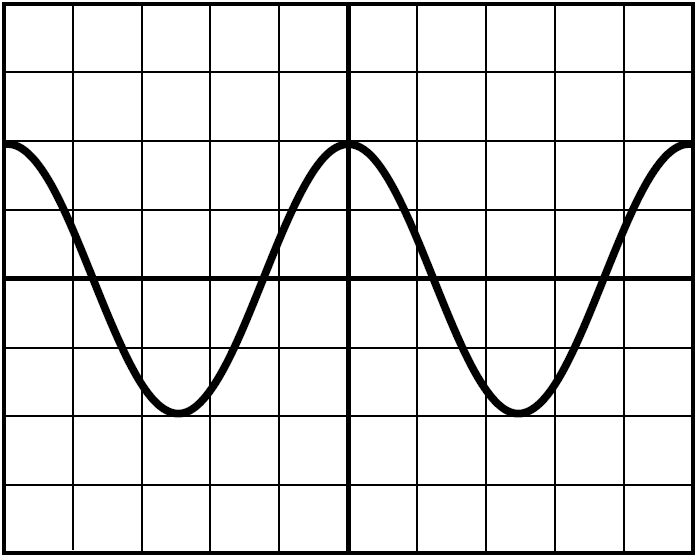
\includegraphics[width=0.4\textwidth]{images/Oszi2.png}

\begin{choices}
	\choice \(\mathrm{250\,Hz}\)
	\choice \(\mathrm{1\,kHz}\)
	\choice \(\mathrm{5\,ms}\)
	\choice \(\mathrm{2,5\,ms}\)
	\choice \(\mathrm{0,5\,ms}\)
\end{choices}

\vspace{3mm}\question Eine Schwingung vollführt in 100 ms genau 10 vollständige Perioden. Wie groß ist die Frequenz?

\begin{choices}
	\choice \(\mathrm{100\,MHz}\)
	\choice \(\mathrm{100\,kHz}\)
	\choice \(\mathrm{100\,Hz}\)
	\choice \(\mathrm{100\,mHz}\)
	\choice \(\mathrm{100\,\mu Hz}\)
\end{choices}

\vspace{3mm}\question Welcher der folgenden Kurvenverläufe gibt den Zusammenhang zwischen der angelegten Spannung und der Kapazität eines Kondensators qualitativ richtig wieder? 

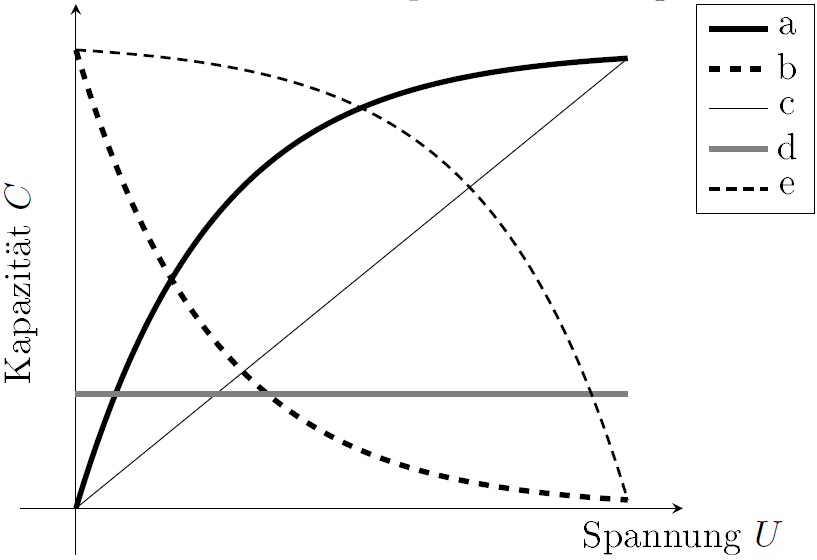
\includegraphics[width=0.4\textwidth]{images/Kondensator-C-U.png}

\begin{choices}
	\choice e
	\choice c
	\choice d
	\choice b
	\choice a
\end{choices}

\vspace{3mm}\end{questions}

\end{document}
